\chapter{Технологический раздел}\label{ch:ch3}
\section{Процесс разработки {\ProgModule}}\label{sec:ch3/sec1}
Разработка {\ProgModule} происходила на языке программирования Nim,
с использованием системы контроля версий git \autocite{git}.

Система контроля версий -- это система, сохраняющая
изменения в файлае или наборе файлов в течение времени и позволяющая возвращаться к их
определенным версиям. 
Это позволяет вернуть файлы в состояние, в котором они были до внесения изменений,
возвратить проект к исходному состоянию, защитить себя и проект от безвозвратной потери
работающей версии программы вследстивие ломающих изменений, удаления или другой утери файлов.
Помимо этого системы контроля версий значительно облегчают параллельную разработку программ,
позволяя нескольким разработчикам одновременно работать в разных <<ветках>> -- 
это специальные указатели на конкретное изменение файлов в системе контроля версий,
которые позволяют добавлять изменения не затрагивая иерархию изменений других веток.
Все это возможно, так как система контроля версий хранит не сами файлы, а лишь
изменения в виде набора <<заплаток>> (патчей, от анг. patch) к ним. Заплатки это небольшие файлы
содержащие только информацию о изменениях, произошедших между стадиями фиксации изменений -- 
<<коммитами>>.

Пример заплатки:
\hspace{-3ex}
\begin{ListingEnv}[!h]
    \captiondelim{ }
    \caption{git diff}\label{lst:diff}
    \small
    \begin{Verb}[]
    diff --git a/analysis/static/aggregation.nim b/analysis/static/aggregation.nim
    index 1623a36..13ac345 100644
    --- a/analysis/static/aggregation.nim
    +++ b/analysis/static/aggregation.nim
    @@ -1,4 +1,4 @@
    -## Этот модуль занимается агреггированием результатов
    +## Этот модуль занимается агрегированием результатов
     ## линковки и статического анализа:
     ## Всем CflowConstruct выставляется ``text_offset`` -- адрес функции в бинарнике
     ##
    \end{Verb}
\end{ListingEnv}

\subsection{Сборка программы на языке Nim}\label{sec:ch3/sec1/sub1}
Язык Nim, как уже говорилось ранее в \autoref{sec:ch2/sec1/sub1/sub3}, для преобразования
исходных кодов использует source-to-source (S2S) компиляцию, а в качестве языка компиляции
используется язык Си, либо JavaScript. Для сборки {\ProgModule} компилятору задаются 
такие параметры, что исходные коды компилируются в Си, ради высокой скорости исполнения
программы.
Компилятор Nim, помимо всего прочего, имеет возможность генерировать документацию, в формате
\verb|.html| и \verb|.json| из файлов с исходным кодом.
Для генерации документации используются комментарии в формате reStructuredText.
Для привязки комментария к функции, типу или определению класса,
комментарий должен быть написан сразу после объявления функции,
типа или определения класса.

\begin{figure}[!hbtp]
    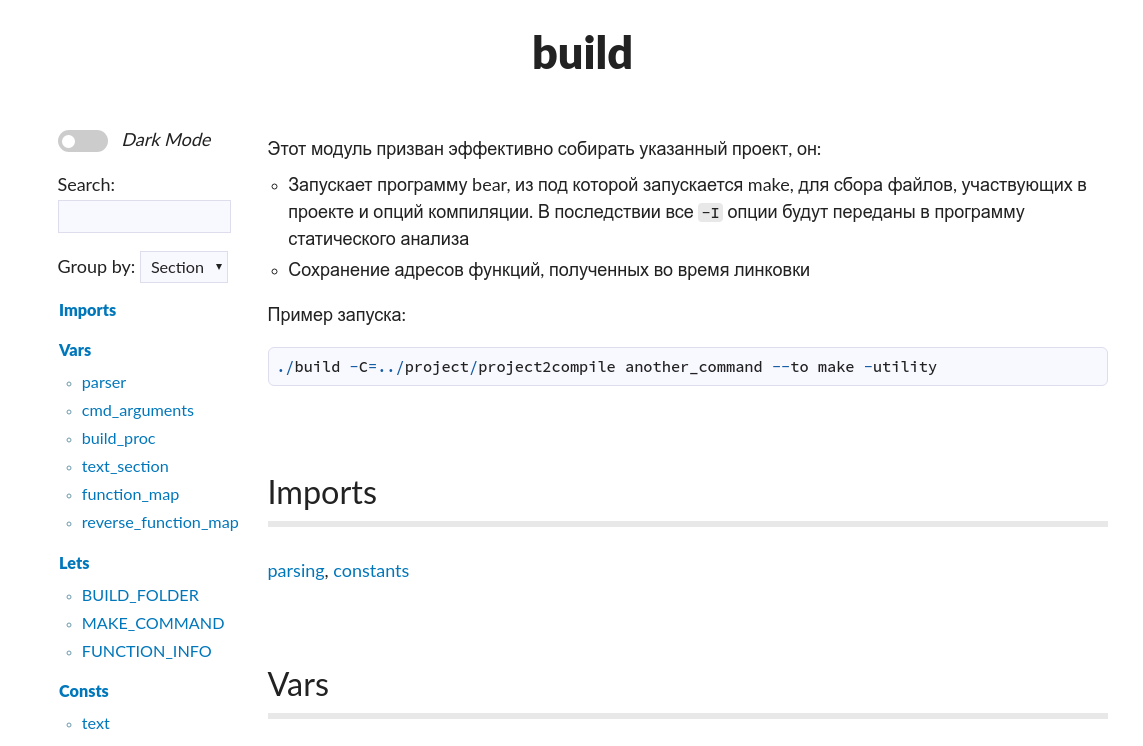
\includegraphics[width=\textwidth,height=\textheight,keepaspectratio]{images/nim_doc_gen.png}
    \caption{Сгенерированная документация по одному из модулей {\ProgModule}\label{fig:nim-doc-gen}}
\end{figure}


В {\ProgModule}, в качестве системы сборки программы используется самописный скрипт на Bash, листинг \autoref{lst:build.sh}, выполняющий следующие действия:
\begin{enumerate}[label={\arabic*)}]
    \item удаляется и создается заново папка \verb|build|, содержащая скомпилированные модули;
    \item текущая папка меняется на \verb|build|;
    \item ищутся все файлы с расширением \verb|.nim|, после чего для каждого файла
        запускается процесс компиляции.
\end{enumerate}

Рассмотрим процесс компиляции. Компилятор запускается со следующими параметрами:
\begin{itemize}
    \item \verb|--parallelBuild:$(nproc)| -- говорит компилятору 
        использовать параллельную компиляцию, с количеством параллельных процессов равному
        количеству процессоров в компьютере;
    \item \verb|--outDir=.| -- файлы, полученные в процессе компиляции, будут сохранены в 
        текущую папку;
    \item \verb|-p=..| -- указывает родительский каталог;
    \item \verb|--threads:on| -- говорит компилятору разрешить компилируемой программе использовать
        механизм потоков, компилятор дополнительно проверяет потокобезопасность программы;
    \item \verb|с $(readlink -f $source_file)| -- говорит компилятору, какой файл компилировать,
        а команда \verb|readlink -f| предоставляет компилятору абсолютный путь до файла в системе.
\end{itemize}

\subsection{Тестирование {\ProgModule}}\label{sec:ch3/sec1/sub2}
Тестирование програмного обеспечение -- это процесс проверки соответствия поведения 
ПО и ожидаемых результатов на некотором множестве тестов. Может проводиться как вручную,
так и с помощью специализированных программ, призванных автоматизировать процесс.
Тестирование может различаться как по типам, так и по методам тестирования.
В {\ProgModule} применялись следующие типы тестирования:
\begin{enumerate}[label={\arabic*)}]
    \item юнит-тестирование -- тестирование модулей {\ProgModule} и их частей;
    \item интеграционное тестирование -- тестирование взаимодействия модулей
        {\ProgModule} между собой;
    \item системное тестирование -- тестирование {\ProgModule} как системы в целом.
\end{enumerate}
Методов тестирования три:
\begin{enumerate}[label={\arabic*)}]
    \item тестирование методом белого ящика -- ПО тестируется с учетом
        работы внутренних механизмов программы;
    \item тестирование методом черного ящика -- ПО тестируется без учета
        работы внутренних механизмов программы;
    \item тестирование методом серого ящика -- ПО тестируется с неполным знанием
        работы внутренних механизмов программы.
\end{enumerate}

{\ProgModule} разрабатывался с использованием техники test-driven development \autocite{TDD} -- разработки через тестирование, или TDD.

\begin{table}
    {\small
        \setlength{\tabcolsep}{2pt}
        \caption{\label{table:testing-comparsion}
            Сравнение методов тестирования для разработки {\ProgModule}}
        \begin{longtable}{*{2}{| c}|}
            \hline
                \makecell{Метод тестирования} & \makecell{Потребность в использовании} \\
            \hline
                \makecell{Метод белого ящика} & \makecell{Нет потребности,\\
                так как {\ProgModule} разрабатывался
                с применением TDD\\ и ориентацией на интерфейс
                между модулями} \\
            \hline
                \makecell{Метод черного ящика} & \makecell{Есть потребность,\\
                 для тестирования корректности работы\\каждого модуля {\ProgModule}} \\
            \hline
                \makecell{Метод серого ящика} & \makecell{Есть потребность,\\
                 для тестирования корректности работы\\связи между модулями {\ProgModule}} \\
            \hline
        \end{longtable}
    }
\end{table}

Разработка через тестирование -- это подход к разработке программного обеспечения, основывающийся
на очень коротком цикле разработки: требования к ПО становятся специальными вариантами тестирования,
а код улучшается до того момента, пока тест не будет проходить успешно. 

Плюсы данного принципа разработки состоят в следующем:
\begin{enumerate}[label={\arabic*)}]
    \item подход помогает разработчикам быть уверенным в коде, который они пишут;
    \item правильное написание тестов позволяет реже использовать отладку для поиска
        ошибок в ПО;
    \item при фокусировании на создании тестовых сценариев, разработчик в первую
        очередь представляет функциональность с позиции клиентов. А значит он будет
        ставить в разработку интерфейса над разработкой функциональности, что
        является еще одним кирпичиком в хорошем дизайне программы.
\end{enumerate}
Такой принцип разработки позволяет не только

Цикл разработки ПО с помощью методологии TDD состоит из следующих шагов:
\begin{enumerate}[label={\arabic*)}]
    \item Добавить тест.\\
        В TDD каждая новая функциональнаость должна начинаться с написания теста для нее.
        Для написания теста разработчик должен хорошо понимать специфику добавляемой 
        функциональности и требования, накладываемые на нее. Это помогает разработчику
        фокусироваться на важных вещах при разработке функционала.
    \item Запустить все тесты и проверить, что новый тест завершился с ошибкой.\\
        Это подтверждает, что все тесты работают корректно, а так же показывает,
        что новый тест не срабатывает без написания нового кода, 
        в случае, если требуемая функциональность уже имеется и исключает 
        возможность некачественного теста.
        Так же этот шаг увеличивает уверенность разработчика в качестве теста.
    \item Написать код.\\
        На этом шаге требуется написать код для вводимой функциональности, который
        заставит тест завершиться успехом. Не обязательно стараться написать код, 
        который будет хорошо работать, качество кода будет повышено на следующих
        шагах.
    \item Запустить все тесты.\\
        Если все тестовые сценарии проходят, то разработчик становится уверенным,
        что код удовлетворяет тестовым требованиям и не ломает текущий функционал ПО.
        Если это не так, то новый код дорабатывается, пока не будут проходить все тесты.
    \item Рефакторинг.\\
        Увеличивающаяся кодовая база должна регулярно подчищаться при использовании TDD.
        Новый код может быть перемещен из мест, где он требовался для срабатывания тестов,
        в место, где он будет более органичен. Постоянно перезапуская тесты во время
        рефакторинга, разработчик может быть уверен, что своими действиями не повлиял на 
        существующую функциональность
    \item Повторение.\\
        Каждый новый тест продвигает функционал не меньше, чем написанный код.
        Шаг, с которым редактируется код и запускается тест всегда должен быть
        маленьким, от 1 до 10 редактирований между запусками.
        Если новый код никак не может удовлетворить требованиям теста, или
        другие тесты перестали проходить, то вместо отладки TDD советует откатить
        внесенные изменения и начать работу заново.
\end{enumerate}

Так как все общение между модулями происходит посредством файлов, то тестированию
подвергался данный интерфейс. Тестирование отдельных методов внутри модулей,
а так же корректность разбора аргументов модулей,
в которых имеется данный интерфейс, производились, но не будут упомянуты
в таблице из-за их примитивности и массовости.

\begin{table}
    {\footnotesize
        \setlength{\tabcolsep}{2pt}
        \caption{\label{table:test-cases}
            Сценарии модульного тестирования {\ProgModule}}
        \begin{longtable}{|c|l|l|}
            \hline
                \makecell{Цель} & \makecell{Ожидаемый результат} & \makecell{Тест} \\
            \hline
                \makecell{Проверить корректность \\
                запуска сборки и сообщение\\ об ошибках сборки} & 
                \makecell[l]{
                    При удачной сборке\\генерируется compilation db,\\
                    лог сборки,\\прямой и обратный map-файл.\\
                    Код возврата модуля сборки равен 0. \\ 
                    \\
                    При неудачной сборке\\
                    генерируется только лог сборки,\\содержащий ошибки.\\
                    Код возврата модуля сборки равен 1.} & 
                \makecell[l]{Тест запускает сборку\\
                трех различных проектов:\\
                не содержащего ошибки,\\
                содержащего ошибки,\\
                пустого проекта.\\
                Проверяется наличие файлов\\
                и код возврата модуля.}\\
            \hline
                \makecell{Проверить корректность \\
                    парсера логов\\динамического анализа} & 
                \makecell[l]{
                    При удачном разборе\\генерируется JSON-файл,\\
                    описывающий процесс.\\
                    Код возврата модуля сборки равен 0. \\ 
                    \\
                    При неудачной сборке\\
                    ничего не генерируется.\\
                    Код возврата модуля сборки равен 1.} & 
                \makecell[l]{Тест запускает парсер на\\
                трех вариантах лога:\\
                не содержащего ошибки,\\
                с нарушеним формата JSON,\\
                пустого файла,\\
                а так же без лога.\\
                Проверяется наличие файла,\\
                описывающего процесс\\
                и код возврата модуля.}\\
            \hline
                \makecell{Проверить корректность \\
                    парсера логов\\динамического анализа} & 
                \makecell[l]{
                    При удачном разборе\\генерируется JSON-файл,\\
                    описывающий процесс.\\
                    Код возврата модуля сборки равен 0.\\
                    \\
                    При неудачной сборке\\
                    ничего не генерируется.\\
                    Код возврата модуля сборки равен 1.} & 
                \makecell[l]{Тест запускает парсер на\\
                    трех вариантах лога:\\
                    не содержащего ошибки,\\
                    с нарушеним формата JSON,\\
                    пустого файла,\\
                    а так же без лога.\\
                    Проверяется наличие файла,\\
                    описывающего процесс\\
                    и код возврата модуля.}\\
            \hline
                \makecell{Проверить корректность \\
                    динамического анализатора} & 
                \makecell[l]{
                    При корректной работе\\
                    генерируется JSON-файл с\\
                    описанием процесса, в котором все\\
                    точки останова стоят\\
                    на call-инструкциях
                    \\
                    При некорректной работе\\
                    хотя бы одна точка останова\\
                    будет стоять не на \\
                    call-инструкции.} & 
                \makecell[l]{Тест запускает парсер\\
                    динамического лога \\
                    и проверяет расположение\\
                    точек останова.}\\
                \hline
        \end{longtable}
    }
\end{table}

\subsection{Профилирование {\ProgModule}}\label{sec:ch3/sec1/sub3}
Профилирование -- вид динамического анализа программы, задачей которого
является измерение характеристик программы во время её выполнения.
Зачастую профилирование служит инструментом для выявления мест 
оптимизации программ. Профилировщики могут измерять количество выделяемой
программе памяти, частоту и время выполнения отдельных функций и др.

При разработке {\ProgModule}, для профилирования использовался
модуль стандартной библиотеки -- \verb|nimprof|. Другое название nimprof --
Embedded Stack Trace Profiler или <<Встроенный профилировщик стека вызовов>>,
которое раскрывает его суть -- профилировщик анализирует стек вызовов и время,
затраченное на выполнение каждой конкретной функции.
Для включения профилировщика, требуется скомпилировать модуль, который будет
профилироваться, с флагами \verb|--profiler:on| и \verb|--stacktrace:on|

Профилировщик работает следующим образом:
во время работы основной программы создаются снимки состояния каждой функции,
а стек вызовов показывает, каким путем дошла прогамма до вызова конкретной 
функции. После окончания работы профилируемой программы генерируется файл
\verb|profile_results.txt|

Рассмотрим формат отчета \autoref{lst:nimprof} профилировщика:
\begin{ListingEnv}[!h]
    \captiondelim{ }
    \caption{Часть лога профилировщика одного из модулей}\label{lst:nimprof}
    \small
    \begin{Verb}[]
total executions of each stack trace:
Entry: 1/157 Calls: 20/249 = 8.03% [sum: 20; 20/249 = 8.03%]
  /toolchains/nim-1.2.0/lib/system/iterators_1.nim: readLine 29/249 = 11.65%
  /toolchains/nim-1.2.0/lib/pure/streams.nim: fsReadLine 21/249 = 8.43%
  /toolchains/nim-1.2.0/lib/pure/streams.nim: readLine 29/249 = 11.65%
  project/breakpoints/parse_log.nim: parse_log 248/249 = 99.60%
Entry: 2/157 Calls: 7/249 = 2.81% [sum: 27; 27/249 = 10.84%]
  /toolchains/nim-1.2.0/lib/system/iterators.nim: escapeJsonUnquoted 21/249 = 8.43%
  /toolchains/nim-1.2.0/lib/pure/json.nim: escapeJson 62/249 = 24.90%
  /toolchains/nim-1.2.0/lib/pure/json.nim: escapeJson 62/249 = 24.90%
  /toolchains/nim-1.2.0/lib/pure/marshal.nim: storeAny 146/249 = 58.63%
  /toolchains/nim-1.2.0/lib/pure/marshal.nim: storeAny 146/249 = 58.63%
  /toolchains/nim-1.2.0/lib/pure/marshal.nim: storeAny 146/249 = 58.63%
  /toolchains/nim-1.2.0/lib/pure/marshal.nim: storeAny 146/249 = 58.63%
  /toolchains/nim-1.2.0/lib/pure/marshal.nim: storeAny 146/249 = 58.63%
  /toolchains/nim-1.2.0/lib/pure/marshal.nim: $$ 146/249 = 58.63%
  project/breakpoints/parse_log.nim: parse_log 248/249 = 99.60%
  ...
Entry: 42/157 Calls: 2/249 = 0.80% [sum: 134; 134/249 = 53.82%]
  /toolchains/nim-1.2.0/lib/system/arithmetics.nim: +% 21/249 = 8.43%
  /toolchains/nim-1.2.0/lib/system/assign.nim: genericAssignAux 25/249 = 10.04%
  /toolchains/nim-1.2.0/lib/system/assign.nim: genericAssign 27/249 = 10.84%
  /toolchains/nim-1.2.0/lib/system/assign.nim: genericSeqAssign 21/249 = 8.43%
  /toolchains/nim-1.2.0/lib/pure/options.nim: some 8/249 = 3.21%
  /toolchains/nim-1.2.0/lib/impure/nre.nim: matchImpl 15/249 = 6.02%
  /toolchains/nim-1.2.0/lib/impure/nre.nim: find 13/249 = 5.22%
  project/breakpoints/parse_log.nim: parse_log 248/249 = 99.60%
  ...
    \end{Verb}
\end{ListingEnv}

Записи в отчете начинаются со слова \verb|Entry|, сразу после него идет номер
записи, количество сделанных вызовов записи в количественном и процентном
соотношении относительно всех вызовов. Внутри квадратных скобок видно, сколько
вызовов и какое покрытие в количественном и процентном соотношении существует на
момент вызова данной функции.
После описания конкретной записи идет описание стека вызовов со статистикой использования 
функций:
\begin{itemize}
    \item \verb|/toolchains/nim-1.2.0/lib/pure/streams.nim:| -- путь до файла, в котором 
        описана функция из стека вызовов;
    \item \verb|fsReadLine| -- имя функции;
    \item \verb|21/249| -- количество вызовов функции относительно всех вызовов;
    \item \verb|= 8.43%| -- процентное соотношение вызовов функции ко всем вызовам.
\end{itemize}

Представленная часть лога \autoref{lst:nimprof} относится к модулю разбора результатов
динамического анализа и по ней видно, что больше всего времени было затрачено на вызов 
функции \verb|readLine| -- 8\% всего времени исполнения модуля,
которая отвечает за чтение строки.
Это логично и объясняется тем, что хотя необработанный файл динамического анализа мал --
в нем содержится всего 25621 строка, операция чтения будет самой частоиспользуемой
из-за назначения профилируемого модуля, а загрузка данных с диска сама по себе
является затратной операцией, не смотря на поддержание библиотекой streams некоего
внутреннего буфера для оптимизации времени получения данных. 

\subsection{Отладка {\ProgModule}}\label{sec:ch3/sec1/sub4}
Параметры компилятора, разобранные ранее, 
позволяют создавать релизную сборку {\ProgModule}.
Для сборки программы с отладочными символами требуется 
указать параметр \verb|--debugger:on|.

Как и тестирование, отладка может проводиться с помощью
различных методов:
\begin{itemize}
    \item интерактивная отладка;
    \item отладочная печать;
    \item post-mortem отладка или отладка <<после смерти>>;
    \item отладка методом <<волчья ограда>>;
    \item отладка методом записи и воспроизведения.
\end{itemize}

\subsubsection{Интерактивная отладка}\label{sec:ch2/sec1/sub3/sub1}
Метод отладки предусматривает запуск отлаживаемой программы в контексте
отладчика, расставление точек останова во время выполнения программы, просмотр
любых переменных окружения, состояние стека вызовов, изменение переменных
для тестирования поведения отлаживаемой программы.
Интерактивные отладчики очень распространены, зачастую тем или иным образом
интегрированы в IDE. Для компилируемых программ требуется наличие отладочных
символов -- специальной информации, генерируемой компилятором при 
преобразовании исходного кода в машинный. В ней содержится информация о 
файле с исходным кодом и позволяет интерактивным отладчикам сопоставлять
блоки машинных инструкций с выражениями языка исходных кодов. Могут
быть как интегрированы в исполняемый файл, так и сохраняться отдельно ввиду
серьезного раздувания размера исполняемых файлов для больших программ.
Одним из первых интерактивных отладчиков был DDT или DEC Debugging Tape,
написанный для PDP-1 в 1964.

\subsubsection{Отладочная печать}\label{sec:ch2/sec1/sub3/sub2}
Самый старый из методов отладки. Иногда его называют <<printf() отладкой>>, 
из-за функции printf() стандартной библиотеки языка Си. Заключается
в выводе, обычно на экран, информации о переменных или выполняющихся
условиях. Несмотря на свою старость, до сих пор является удобным способом 
отладки программный проектов при должном количестве выводимой информации.
Результаты отладки могут быть направлены в файл, для последующего внимательного
разбора.

\subsubsection{Отладка <<после смерти>>}\label{sec:ch2/sec1/sub3/sub3}
Отладка программы после того, как программа неисправимо сломалась.
Суть постмортем отладки заключается в анализе логов, просмотра состояния
стека вызовов и слепка памяти на момент появления исключительной ситуации.

\subsubsection{Отладка методом <<волчья ограда>>}\label{sec:ch2/sec1/sub3/sub4}
Или методом бисекции. Впервые описан в журнале ACM \autocite{wolf-fence}. 
Суть метода заключается в нахождении места ошибки через отсечение корректно
работающих областей кода до момента, пока разработчик не попадет на некорректно
работающую область. Удобно применять вместе с просмотром стека вызовов до момента
происхождения исключительной ситуации. Яркий пример применения -- команда
\verb|git bisect|, позволяющая быстро найти коммит, в котором впервые
появилась ошибка.

\subsubsection{Отладка методом записи и воспроизведения}\label{sec:ch2/sec1/sub3/sub5}
Данный тип отладки подразумевает предварительную запись работы
программы и последующее отлаживание уже сделанной записи.
Это позволяет лучше исследовать причины ошибки, а так же отлавливать и анализировать
трудновоспроизводимые ситуации, появляющиеся, например, из-за случайных событий.
\\

При разработке {\ProgModule}, не смотря на то, что TDD рекомендует писать тесты
при любой ошибке, а не заходить в отладчик, комбинирование обоих подходов
повышает производительность разработчика, так как в одних ситуациях
удобнее и быстрее всего отладить совсем небольшую ошибку, а не писать для нее тест
и запускать после этого все тесты модуля. Данная практика является
наиболее распространенной среди разработчиков, применяющих TDD.
Из всех перечисленных методов, для отладки {\ProgModule} использовалось два: отладочная
печать и интерактивная отладка. Отладочная печать была удобна при внесении изменений
между тестами, так как дополняла их результаты, а интерактивная отладка при анализе
процесса исполнения {\ProgModule}. Для интерактивной отладки использовался отладчик 
GDB \autoref{fig:running-gdb}.

\begin{figure}[!hbtp]
    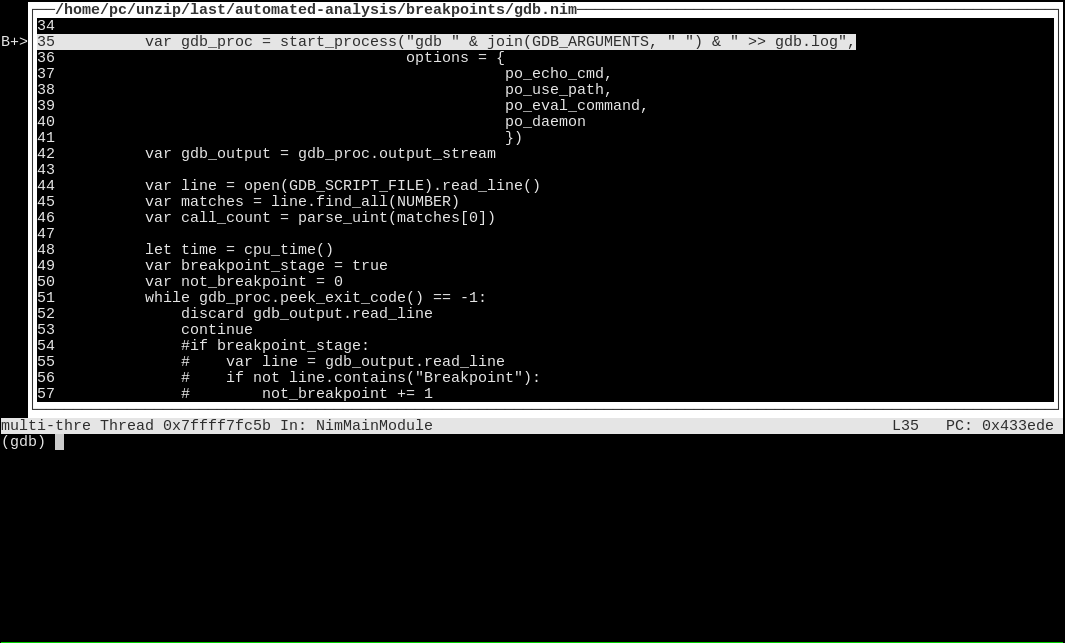
\includegraphics[width=\textwidth,height=\textheight,keepaspectratio]{images/running-gdb.png}
    \caption{Отладка {\ProgModule} в GDB\label{fig:running-gdb}}
\end{figure}

На \autoref{fig:running-gdb} можно увидеть терминальный интерфейс отладчика. Он
запускается передачей GDB аргумента \verb|-tui|, или выполнением команды 
\verb|layout next| из командного интерфейса GDB.
Это не единственный вид интерфейса, который предоставляет GDB.
Есть, например, \verb|split| интерфейс \autoref{fig:layout-split},
который позволяет одновременно видеть, как исполняемые машинные инструкции,
так и исходный код программы.

Независимо от выбранного интерфейса, GDB оставляет командную строку для 
управления процессом отладки, которая обязательно начинается с \verb|(gdb)|.
Через нее происходит управление отладчиком -- установка точек останова,
просмотр адресов памяти, переменных, изменение значений.
GDB имеет большое количество команд значительно облегчающих отладку программ, 
а на их основе можно сделать мета-команды, объединяющие функционал нескольких
команд.

\begin{figure}[!hbtp]
    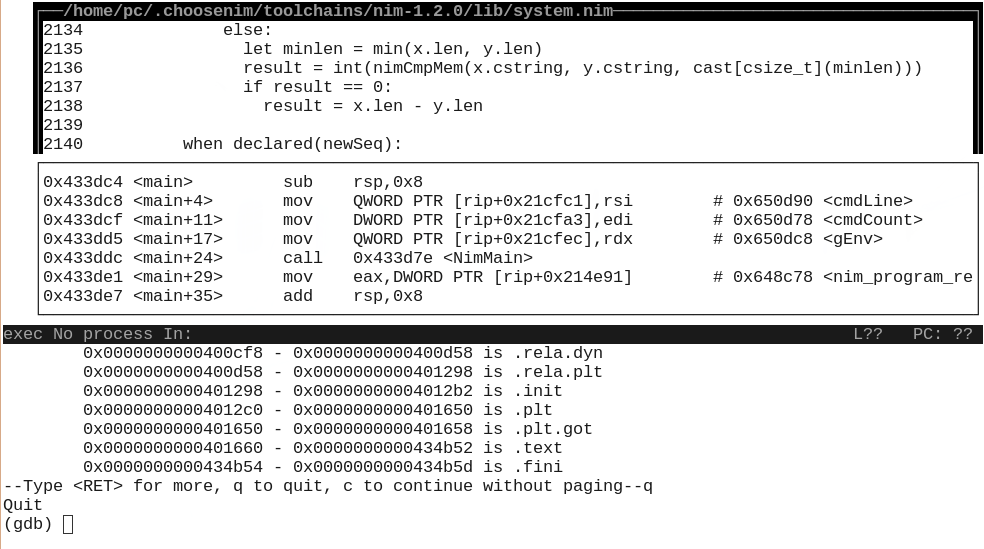
\includegraphics[width=\textwidth,height=\textheight,keepaspectratio]{images/split-layout.png}
    \caption{layout split в GDB\label{fig:layout-split}}
\end{figure}

Начать отлаживать любую программу в GDB можно двумя способами:
\begin{itemize}
    \item запустить отладчик передав ему в качестве аргумента путь до отлаживаемого файла;
    \item подключиться к уже работающему процессу.
\end{itemize}

При как при отладке процесса, так и исполняемого файла GDB
запустится с приветствием, содержащим версию и год, в который она была выпущена,
а так же попытается найти отладочные символы не только для отлаживаемого процесса или файла, 
но и для используемых динамических библиотек (если таковые используются программой),
пример в листинге \autoref{lst:gdb-bash}.
Если же отладочные символы не нашлись, то GDB сообщит об этом:
\verb|(No debugging symbols found in имя-файла)|

\begin{ListingEnv}[!h]
    \captiondelim{ }
    \caption{Отладка Bash}\label{lst:gdb-bash}
    \small
    \begin{Verb}[]
        Attaching to process 16108
        Reading symbols from /bin/bash...
        Reading symbols from /lib/x86_64-linux-gnu/libtinfo.so.5...
        Reading symbols from /lib/x86_64-linux-gnu/libdl.so.2...
        (No debugging symbols found in /lib/x86_64-linux-gnu/libdl.so.2)
        Reading symbols from /lib/x86_64-linux-gnu/libc.so.6...
        (No debugging symbols found in /lib/x86_64-linux-gnu/libc.so.6)
    \end{Verb}
\end{ListingEnv}
